\chapter{Challenges with Collaborative Text Editing} \label{chapter:challenges}

This chapter first introduces the goal of user intent-preservation by showing the problem of text interleaving in \Cref{section:challenges-text-interleaving}. Then, \Cref{section:challenges-text-interleaving-fugue} introduces the solution proposed by Fugue \cite{2023-weidner-minimizing-interleaving} to solve text interleaving. Finally, \Cref{chapter:ot} compares \glspl{crdt} and \gls{ot} and shows that the current \glspl{crdt} runtime complexity is quadratic and current \gls{ot} algorithms are unsuitable for \textit{non-realtime} editing.

\section{Text Interleaving} \label{section:challenges-text-interleaving}

When users write text in a collaborative text editor, they expect that their text is not modified in an unexpected way by concurrent edits from other users. One example are insertions at \textit{different} positions. Starting with the text \texttt{"Alice plays Minecraft"}, \textcolor{red}{Alice} changes the text to \texttt{"Alice \textcolor{red}{happily} plays Minecraft"}. Concurrently, \textcolor{blue}{Bob} changes the text to \texttt{"Alice plays Minecraft \textcolor{blue}{with Bob}"}. Then, the expected result after synchronizing is \texttt{"Alice \textcolor{red}{happily} plays Minecraft \textcolor{blue}{with Bob}"}. As the insertions are at different positions in the text, the expected outcome is unambiguous, and all characters should stay at their relative position to the surrounding characters.
Users also expect that text they wrote in one go is not interleaved by text that another user wrote concurrently. An example with insertions at the \textit{same} position is the following. Starting with the text \texttt{"milk, chocolate"}, \textcolor{red}{Alice} changes the text to \texttt{"milk, \textcolor{red}{eggs,} chocolate"} and \textcolor{blue}{Bob} concurrently changes the text to \texttt{"milk, \textcolor{blue}{bread,} chocolate"}. The expected result after synchronizing is either \texttt{"milk, \textcolor{red}{eggs,} \textcolor{blue}{bread,} chocolate"} or \texttt{"milk, \textcolor{blue}{bread,} \textcolor{red}{eggs,} chocolate"}. While there are two possibilities in this case, no interleaving occurs in either case.

\begin{figure}
  \centering
  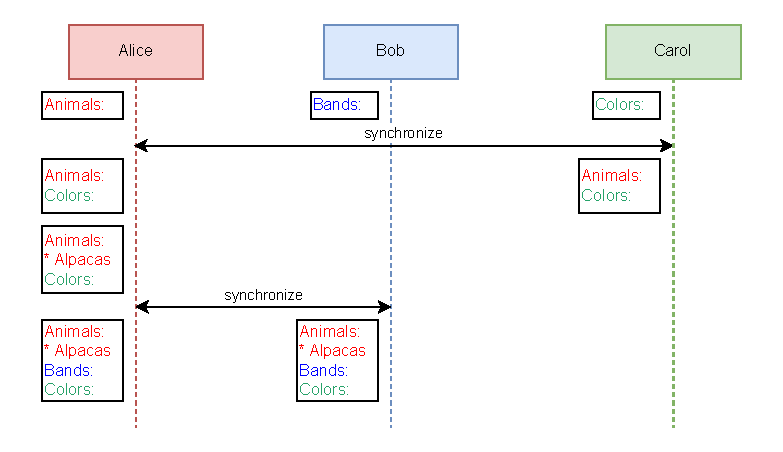
\includegraphics[width=\textwidth]{figures/forward-more-important-than-backward.drawio.pdf}
  \caption{Example for prioritizing forward insertions inspired by Figure 6 in Fugue \protect\cite{2023-weidner-minimizing-interleaving}}
  \label{fig:forward-more-important-than-backward}
\end{figure}

\clearpage

For an insertion in the middle of a text, current editing behavior does not convey whether the insertion semantically belongs to the left side or the right side. Because most text is written in a forward direction, so for left-to-right script from left to right, it is more likely that an insertion in the middle of some text is appending to the left side of the insertion point instead of prepending to the right side of the insertion point. \Cref{fig:forward-more-important-than-backward} exemplifies this. The three replicas \textcolor{red}{Alice}, \textcolor{blue}{Bob} and \textcolor{mygreen}{Carol} independently add three lists to some text. Then, \textcolor{red}{Alice} and \textcolor{mygreen}{Carol} synchronize. Afterwards, \textcolor{red}{Alice} adds \texttt{"\textcolor{red}{*~Alpacas}"} to her list, such that it comes after \texttt{"\textcolor{red}{Animals:}"} and before \texttt{"\textcolor{mygreen}{Colors:}"} but inherently there is no information to which part it belongs. Finally, \textcolor{red}{Alice} and \textcolor{blue}{Bob} synchronize. This separates \texttt{"\textcolor{red}{*~Alpacas}"} and \texttt{"\textcolor{mygreen}{Colors:}"} by the received \texttt{"\textcolor{blue}{Bands:}"}, which may not be wanted. In this example the assumption of the more common forward insertion is correct though. Further improvements to this would need analysis of the language semantics of the text which \Citeauthor*{2023-bauwens-nlp-for-merging} looked into \cite{2023-bauwens-nlp-for-merging}. For the concrete example, a different idea could be to insert \texttt{"\textcolor{blue}{Bands:}"} after \texttt{"\textcolor{mygreen}{Colors:}"} so \texttt{"\textcolor{red}{*~Alpacas}"} stays in place in relation to the text preceding and following it. Unfortunately this would lead to even more unexpected behavior for example when \textcolor{blue}{Bob} and \textcolor{mygreen}{Carol} synchronized before and would order the entries alphabetically because they do not know about the insertion of \texttt{"\textcolor{red}{*~Alpacas}"}. As soon as \textcolor{red}{Alice} would then synchronize with them, the entries would need to be reordered, so that they converge. As the synchronized data is not structured like the example may suggest, but instead consists of arbitrary characters, this reordering could result in sentence reordering or other unwanted results. Another idea could be to prefer the side by the same replica. This has similar issues if concurrent edits are received later and change the effect of that rule.

\section{Fugues Approach to Avoid Text Interleaving} \label{section:challenges-text-interleaving-fugue}

This section shows the proposed solution by Fugue \cite{2023-weidner-minimizing-interleaving} to solve text interleaving. It also gives an example that the proposed \textit{maximally non-interleaving} property can still interleave text when deletions are involved.

\Citeauthor*{2023-weidner-minimizing-interleaving} \cite{2023-weidner-minimizing-interleaving} show that a previous attempt at formalizing a property for non-interleaving by \Citeauthor*{2019-Kleppmann-incorrect-noninterleaving-property} \cite{2019-Kleppmann-incorrect-noninterleaving-property} is incorrect \cite[Section 2.5]{2023-weidner-minimizing-interleaving}. Therefore, they propose their own property which they refer to as \textit{maximally non-interleaving}. It associates every inserted character with the character to its left and right, which they label left and right origin. The property orders the characters by prioritizing keeping the left origin as the previous character because of the common forward insertions and otherwise ordering to preserve the right origin as the following character if possible. Only if both origins are the same, the order is arbitrary but deterministically chosen. Therefore, this property creates a unique order aside from tie-breaking \cite[Section 4.5]{2023-weidner-minimizing-interleaving}.

Fugue refers to an interleaving issue as forward interleaving, when only one character has another character as a left origin, yet the two characters are not consecutive. One example where the Logoot algorithm \cite{2009-weiss-logoot} interleaved characters, which also violates this rule, is concurrently inserting \texttt{"\textcolor{blue}{bread}"} and \texttt{"\textcolor{red}{eggs}"}, producing \texttt{"\textcolor{blue}{b}\textcolor{red}{e}\textcolor{blue}{r}\textcolor{red}{g}\textcolor{blue}{e}\textcolor{red}{g}\textcolor{blue}{a}\textcolor{red}{s}\textcolor{blue}{d}"} \cite[Section 4.4.1]{2019-sun-difference-ot-crdt-2-correctness-complexity}. For example the \texttt{"\textcolor{blue}{r}"} from \texttt{"\textcolor{blue}{bread}"} has the \texttt{"\textcolor{blue}{b}"} as its left origin and no other character has the \texttt{"\textcolor{blue}{b}"} as its left origin but in the result they are not consecutive characters.

\Citeauthor*{2023-weidner-minimizing-interleaving} refer to another problem that many prior algorithms exhibit as backward interleaving. When two insertions have the same left origin but a different right origin, they should be ordered in a way that they are consecutive with their right origins. Although it may seem this is not a common use case, the following is a plausible example \cite[Figure 2]{2023-weidner-minimizing-interleaving}. Starting with the text \texttt{"Shopping"}, \textcolor{red}{Alice} first appends \texttt{"\textcolor{red}{*~apples}"} after \texttt{"Shopping"} and then prepends \texttt{"\textcolor{red}{Fruit:}"} before \texttt{"\textcolor{red}{*~apples}"}. While semantically she is prepending, both inserted texts have \texttt{"Shopping"} as their left origin and different right origins. Concurrently, \textcolor{blue}{Bob} first appends \texttt{"\textcolor{blue}{*~bread}"} after \texttt{"Shopping"} and then prepends \texttt{"\textcolor{blue}{Bakery:}"} before \texttt{"\textcolor{blue}{*~bread}"}. The category insertions by \textcolor{red}{Alice} and \textcolor{blue}{Bob} both have \texttt{"Shopping"} as their left origin but different right origins. Therefore, this should lead to either the outcome of \texttt{"Shopping\textcolor{red}{Fruit:*~apples}\textcolor{blue}{Bakery:*~bread}"} or \texttt{"Shopping\textcolor{blue}{Bakery:*~bread}\textcolor{red}{Fruit:*~apples}"} which only differ in the order of which users text comes first, which is arbitrary. When algorithms exhibit backward interleaving, \texttt{"Shopping\textcolor{blue}{Bakery:}\textcolor{red}{Fruit:}\textcolor{blue}{*~bread}\textcolor{red}{*~apples}"} can be a possible result.
Note that the order of the elements has not changed in relation to each other (e.g. \texttt{"\textcolor{red}{Fruit:}"} comes before \texttt{"\textcolor{red}{*~apples}"} and after \texttt{"Shopping"}) but this still violates the intent of the user.

According to \Citeauthor*{2023-weidner-minimizing-interleaving}, many popular algorithms they looked into exhibit either forward or backward interleaving \cite[Table 1]{2023-weidner-minimizing-interleaving}. A review by \Citeauthor*{2023-sun-critical-examination-fugue-ot} \cite{2023-sun-critical-examination-fugue-ot,2023-sun-critical-examination-fugue-ot-1,2023-sun-critical-examination-fugue-ot-2,2023-sun-critical-examination-fugue-ot-3} that refutes these claims for OT algorithms is addressed in \Cref{chapter:ot}. For Logoot \cite{2009-weiss-logoot} the character-by-character interleaving issue occurs. Further examples are provided in the appendix of the Fugue paper \cite{2023-weidner-minimizing-interleaving}. While the prior \gls{crdt} algorithms YjsMod\footnote{\url{https://github.com/josephg/reference-crdts}} and Sync9\footnote{\url{https://braid.org/sync9}} do not exhibit interleaving \cite[Table 1]{2023-weidner-minimizing-interleaving}, those approaches were not considered here due to the lack of documentation and their intrinsic complexity. \Citeauthor*{2023-weidner-minimizing-interleaving} propose their own algorithms Fugue and FugueMax to solve these problems. They conjecture that Sync9 is semantically equivalent to Fugue and YjsMod is semantically equivalent to FugueMax \cite[Section 6]{2023-weidner-minimizing-interleaving}. They also prove that FugueMax fulfills the \textit{maximally non-interleaving} property \cite[Theorem 9]{2023-weidner-minimizing-interleaving}, prove that the Fugue algorithm is always forward non-interleaving \cite[Lemma 7]{2023-weidner-minimizing-interleaving} and argue that it is also backward non-interleaving when there are not multiple interacting concurrent updates \cite[Section 4.3]{2023-weidner-minimizing-interleaving}.

A counter example that interleaving can also happen for the \textit{maximally non-interleaving} FugueMax algorithm is the following. Starting with the text \texttt{"Shopping"}, \textcolor{red}{Alice} appends \texttt{"\textcolor{red}{*~apples}"} after \texttt{"Shopping"} and then prepends \texttt{"\textcolor{red}{Fruit:}"} before \texttt{"\textcolor{red}{*~apples}"}. Concurrently, \textcolor{blue}{Bob} appends \texttt{"\textcolor{blue}{*~bread}"} after \texttt{"Shopping"}, then deletes and reinserts the \texttt{"\textcolor{blue}{g}"} of \texttt{"Shopping"} and finally prepends \texttt{"\textcolor{blue}{Bakery:}"} before \texttt{"\textcolor{blue}{*~bread}"}. The expected result would be \texttt{"Shoppin\textcolor{blue}{gBakery:*~bread}\textcolor{red}{Fruit:*~apples}"} but the actual result can be \texttt{"Shoppin\textcolor{blue}{gBakery:}\textcolor{red}{Fruit:*~apples}\textcolor{blue}{*~bread}"} when the replicas IDs have a specific order. The code in \Cref{appendix:code-fuguemax-interleaving} verifies this with the reference implementation\footnote{\url{https://github.com/mweidner037/fugue}}. The reason the \textit{maximally non-interleaving} property does not cover this case is that it disregards deletions. This example shows that this simplification is not suitable to ensure non-interleaving.

The basic implementation of Fugue has a linear runtime per character insertion or deletion in relation to the text length (including deleted text) which proved to be too inefficient for larger text given the resulting runtime scales quadratically with the text length. Comparing the results\footnote{\url{https://github.com/mweidner037/fugue/blob/main/results_table.md}} from \Citeauthor*{2023-weidner-minimizing-interleaving} for benchmark B1.1 with benchmark B1.3 indicates, that even the optimized variant in the Fugue paper has quadratic runtime for sequential backward insertions.

\clearpage

\begin{figure}
  \centering
  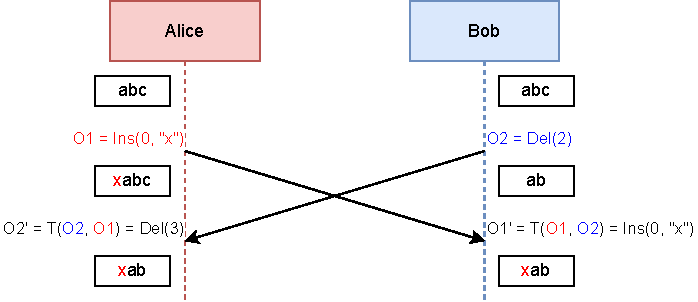
\includegraphics[width=\textwidth]{figures/ot.drawio.pdf}
  \caption{Example for operation transformation with two synchronizing peers based on figure by \Citeauthor*{2024-sun-ot-faq} \cite[Section 1.4 Figure 1]{2024-sun-ot-faq}}
  \label{fig:ot-example}
\end{figure}

\begin{listing}
  \begin{minted}{text}
Tii(Ins[p1,c1], Ins[p2, c2]) {
  if p1 < p2 or (p1 = p2 and u1 > u2)
    return Ins[p1, c1];              
  else
    return Ins[p1+1, c1];
}
\end{minted}
  \caption{Example for transformation function from Sun \cite[Section 2.15]{2024-sun-ot-faq}}
  \label{lst:example-transformation-function}
\end{listing}

\clearpage

\section{OT in Comparison to CRDTs} \label{chapter:ot}

This section explains the differences and similarities between \gls{ot} and \glspl{crdt} and shows that the current \glspl{crdt} runtime complexity is quadratic and current \gls{ot} algorithms are unsuitable for \textit{non-realtime} editing.

While \gls{crdt} papers often claim \glspl{crdt} are superior to \gls{ot}, \glspl{crdt} often miss major relevant parts of the required algorithmic steps which makes them seem potentially simpler and more performant \cite[page 2]{2019-sun-difference-ot-crdt-1-general-transformation-framework}. For example, \glspl{crdt} need to extract the text from their internal state and need to be able to address characters based on their text position as most text editors work that way \cite[Section 5.1, Section 5.2]{2019-sun-difference-ot-crdt-1-general-transformation-framework}. \Glspl{crdt} often miss this conversion step which is a major algorithmic complication that also affects their performance a lot \cite[page 2]{2019-sun-difference-ot-crdt-1-general-transformation-framework}. Note that Fugue also has this issue as it does not describe converting the received operations to character offsets \cite[Algorithm 1]{2023-weidner-minimizing-interleaving}.

\Citeauthor*{2019-sun-difference-ot-crdt-1-general-transformation-framework} also show that both approaches are more similar than often presented \cite[Section 4.1 Table 1]{2019-sun-difference-ot-crdt-1-general-transformation-framework}. While \glspl{ot} have position based operations directly on the character sequence that are then transformed by concurrent operations, \glspl{crdt} have identifier based operations on an internal object sequence, that are converted to the position based character sequence after the operations have been applied.

\gls{ot} based algorithms consist of a control algorithm and a transformation function \cite{2024-sun-ot-faq}. The control algorithm is generic, and the transformation function is application specific. For example for plain text editing there could be two operations, Insert(index, character) and Delete(index). The transformation function $T(O_2, O_1)$ transforms $O_2$ against $O_1$. This produces the operation that needs to be applied after $O_1$ if they were concurrent before. \Cref{fig:ot-example} shows an example where the positions of the concurrent operations are transformed when receiving them and therefore result in the same text at both peers. In that example the transformation function could be defined as shown in \Cref{lst:example-transformation-function} for transforming two insert operations \cite[Section 2.15]{2024-sun-ot-faq}. If a concurrent insertion happened at a position after the current insertion it does not need to be transformed. If a concurrent insertion happened at a position before the current insertion it needs to be offset by one. For equal positions, tie breaking using the replica identifier is required.

The control algorithms decide in which order operations need to be transformed to achieve the desired outcome \cite[Section 2.2]{2024-sun-ot-faq}. Depending on the control algorithm, the transformation function needs to fulfill different properties to ensure correctness \cite[Section 2.20]{2024-sun-ot-faq}. Also, some control algorithms are able to handle undo, some can undo arbitrary actions out of order, while some cannot \cite[Section 2.12]{2024-sun-ot-faq}.

Transformation functions need to be defined for all possible combinations of operations. This means $N^2$ such functions are needed for $N$ possible operations. An alternative proposed by \Citeauthor*{2019-sun-difference-ot-crdt-3-building-real-world-applications} is POT+COA (Primitive Operation
Transformation plus Complex Operation Adaptation). It consists of having some primitive operations for which transformation functions are defined, and then complex application operations are converted to these primitive operations \cite[Section 2.1.3]{2019-sun-difference-ot-crdt-3-building-real-world-applications}.

OT based algorithms can be integrated into existing editors with little change of the editors source code as OT is operation and concurrency-centric. The algorithm can just apply the received and transformed operations to the local editor and send local operations to other peers. \Citeauthor*{2019-sun-difference-ot-crdt-3-building-real-world-applications} refer to this as Transparent Adaptation (TA) \cite[Section 2.1.2]{2019-sun-difference-ot-crdt-3-building-real-world-applications}.

According to \Citeauthor*{2019-sun-difference-ot-crdt-1-general-transformation-framework}, \gls{ot} uses a concurrency-centric and direct transformation approach and \gls{crdt} uses a content-centric and indirect transformation approach \cite[Section 1]{2019-sun-difference-ot-crdt-1-general-transformation-framework}. This has an important consequence for the time and space complexity. The time and space complexity of \gls{ot} for \textit{realtime} editing depends on the number of concurrent operations which are usually small in realtime text editing while the time and space complexity of \gls{crdt} depends on the length of the text or even the length of the text including all deleted content which are usually a lot larger \cite[Section 5.3]{2019-sun-difference-ot-crdt-1-general-transformation-framework}. The time complexity for prior \gls{ot} based algorithms is at least $O(c)$ per remote operation \cite[Section 3.1.4]{2019-sun-difference-ot-crdt-2-correctness-complexity}. This means quadratic runtime complexity in relation to the operation count for handling some count of operations, which is unusable for \textit{non-realtime} editing because there can be many concurrent operations. It is important to mention that the time complexity class is relevant. For example, $O(\log(\text{text-length-including-deletions}))$ runtime complexity can be equally acceptable to $O(\text{concurrent-operations})$ runtime complexity because $O(\log(n))$ is growing quite slowly even for extremely large inputs. Prior research of \glspl{crdt} mostly managed a linear time complexity or worse except of a paper by \Citeauthor*{2016-briot-logn-optimization} which optimizes an \gls{rga} adaptation to $O(\log(n))$ per operation similarly to us \cite[Table 4]{2019-sun-difference-ot-crdt-2-correctness-complexity}. However, \Citeauthor*{2016-briot-logn-optimization} have not gone into the analysis of performance edge cases prohibiting us from drawing a fair comparison. Additionally, it is unclear whether they include the conversion of remote operations to character positions. Furthermore, as the algorithm is based on \gls{rga}, it exhibits interleaving \cite[Table 1]{2023-weidner-minimizing-interleaving}.

While \glspl{crdt} often seem to be simple and easy to understand, the fundamental concurrency issues which are inherent to unconstrained co-editing also exist there and mixing content and concurrency creates new difficulties with handling them \cite[Section~4]{2019-sun-difference-ot-crdt-2-correctness-complexity}.
